\section{Experiment Results}
\label{sec:results}

Each result uses the response RTT and deadline-completion definitions from
Section~\ref{sec:setup} and the application conditions in
Table~\ref{tab:application-envelopes}. The analysis first establishes IPI
workload coverage and direct-PC5 behavior. It then examines 5G uplink payloads,
transport, and stationary radio conditions, followed by downlink-heavy
workloads and two TDD configurations. The final
experiments add sustained streams, concurrent clients, and interruption. This
order separates single-path limits from the conditions that place several CAV
flows on the same network.

\subsection{IPI Workload Representation and Framing Cost}
\label{sec:results-functional}

Before measuring either communication path, we quantify how IPI represents the
two workload classes and how many bytes the representation adds. The message
profile preserves typed BSM, PSM, MAP, SPaT, SRM, and SSM content and a
byte-exact pre-encoded Traveler Information Message (TIM). The operation profile
represents requests, updates, completions, and rejections with session and
correlation information.

Table~\ref{tab:ipi-validation} reports the IPI content representation before
path-specific experiment and transport frames. A preserved J2735 payload of
size $P$~B receives a 1-B type field and a 4-B length field. The CAV rows contain
a planning request and, when present, an opaque application object.

\begin{table}[t]
  \caption{Measured IPI content representation for compact J2735 messages and
  correlated CAV planning operations.}
  \label{tab:ipi-validation}
  \centering
  \scriptsize
  \setlength{\tabcolsep}{2.0pt}
  \begin{tabular}{@{}p{0.40\columnwidth}C{0.16\columnwidth}C{0.17\columnwidth}C{0.18\columnwidth}@{}}
    \toprule
    IPI profile and workload & IPI fields (B) & Content (B) & Total (B) \\
    \midrule
    CV message: preserved J2735 & 5 & $P$ & $P+5$ \\
    CAV operation: planning request & 63 & 0 & 63 \\
    CAV operation: request + object & 78--81 & 256 & 334--337 \\
    CAV operation: request + object & 78--81 & 1,024 & 1,102--1,105 \\
    CAV operation: request + object & 78--81 & 4,096 & 4,174--4,177 \\
    \bottomrule
  \end{tabular}
\end{table}

Each CAV object-size condition contains 1,000 encoded sender records. Their IPI
fields encode the session and vehicle identifiers, service class and status,
request horizon, planning waypoint, confidence, and task identifier. These
fields occupy 78--81~B when a request carries an object. Their share of the
encoded frame therefore decreases from 30.5--31.6\% with a 256-B object to
7.6--7.9\% with a 1-KiB object and 1.9--2.0\% with a 4-KiB object. The added
representation remains fixed or bounded instead of growing with the application
object. Consequently, application content accounts for more than 92\% of the
encoded size at 1~KiB and more than 98\% at 4~KiB. IPI therefore carries
existing compact messages with a 5-B wrapper and adds the operation fields
needed by CAV applications without materially increasing these larger objects.

The binding and experiment frames add path-specific fields beyond the
representations in Table~\ref{tab:ipi-validation}. The July 3--4 PC5 campaign
reports complete serialized frame size. Its nonzero
settings configure 256-, 512-, 1,024-, and 2,048-B IPI performance frames for
submission to the vendor packet-data interface. Every retained nonzero sender
record has a packet length equal to its configured frame size. The zero control
retains the required IPI identity and timing fields and therefore produces a
51--55-B request. The PC5 analysis below varies this complete IPI frame size.
The Uu analyses instead vary application-object size before IPI serialization,
with encoded frame size retained in the sender records. These definitions
separate the application object, IPI representation, and complete transmitted
frame. The field campaigns then exercise IPI through the PC5 custom-data binding
and the Uu TCP, MQTT, and UDP measurement adapters.

\begin{figure*}[t]
  \centering
  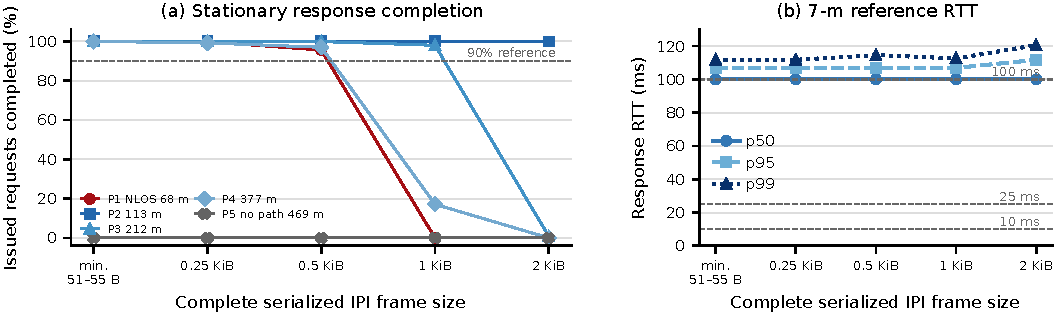
\includegraphics[width=\textwidth]{figs/section5_pc5_payload_route.pdf}
  \caption{Stationary PC5 frame-size results. The response-completion rate is the
  percentage of issued requests that received a sequence-matched response
  before timeout. (a) Completion for the minimum-header control and complete
  serialized IPI frames from 0.25 to 2~KiB at P1--P5; P1 is the
  building-obstructed non-line-of-sight point.
  (b) Response p50, p95, and p99 RTT in a separate 7-m reference collection.}
  \Description{Two plots show stationary PC5 response completion for the
  minimum-header control and complete serialized IPI frame sizes across field
  points, together with response latency at a separate reference point.}
  \label{fig:pc5-results}
\end{figure*}

\subsection{Direct PC5 Stationary Frame-Size Limits}
\label{sec:results-pc5}

The representation results establish the bytes added before a path binding. The
PC5 experiments next measure how complete serialized frame size and field
position affect the exchange across stationary points.
Figure~\ref{fig:pc5-results}(a) compares response completion as
the configured IPI frame size and stationary field point change. P1 is
building-obstructed at 68~m;
P2--P5 are 113, 212, 377, and 469~m from the RSU. The RTT panel uses a separate
7-m reference collection. In that collection, 0.25~KiB
returned 999/1,000 responses; 0.5--2~KiB returned every response. Their p50
RTTs remained near 100~ms. Their p95 RTTs ranged from 106.694 to 111.663~ms
(Figure~\ref{fig:pc5-results}(b)). These RTTs exceed the 10- and 25-ms
cooperative budgets at the median and the 100-ms warning budget at p95.

The effect of frame size increased across the later field points. The 2-KiB failure rate
rose from 0.2\% to 99.2\%, followed by 910 failures before the next collection
was stopped. Over the same sequence, the 1-KiB failure rate rose from 0\% to
2.1\% and then 82.9\%. The 0.25- and 0.5-KiB conditions remained available at
more points. The final point returned no response for any configured frame
size. The nearby
non-line-of-sight (NLOS) point was obstructed by a building and is shown
separately from the ordered field sequence.

\begin{figure*}[t]
  \centering
  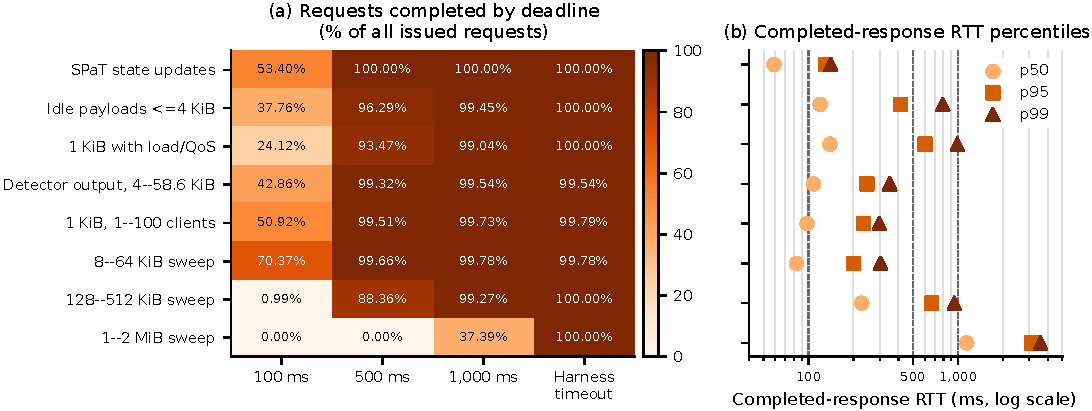
\includegraphics[width=\textwidth]{figs/section5_5g_deadline_envelope.pdf}
  \caption{Uplink-heavy private 5G IPI payload-size and deadline results. The
  vehicle sends the stated workload payload, and d1 returns a compact
  acknowledgment after decoding it. (a) Percentage of all issued requests
  completed within 100, 500, and 1,000~ms and before timeout.
  Detector output denotes serialized object-detection result sizes from 4 to
  58.6~KiB replayed as IPI payloads. (b) The p50, p95, and p99 RTT among
  completed responses.}
  \Description{A heatmap shows the percentage of issued requests completed by
  three deadlines and the timeout for eight named workload groups. A
  dot plot shows response p50, p95, and p99 round-trip time in milliseconds on
  a logarithmic scale.}
  \label{fig:5g-deadlines}
\end{figure*}

\subsection{5G Uplink: Payload Size and Deadlines}
\label{sec:results-5g-payload}

The PC5 measurements expose stationary frame-size and coverage limits for direct
exchange. The
5G evaluation extends the payload range over the network-assisted Uu path.
Each 5G application probe transmits an IPI cooperative-service workload frame
from the vehicle. The d1 endpoint decodes each frame and immediately returns a
compact correlated acknowledgment.
Figure~\ref{fig:5g-deadlines} compares workload responses at 100, 500, and
1,000~ms. Across the eight disjoint workload groups, the analysis contains
752,200 issued requests. Requests with payloads of at most 4~KiB returned
all 60,000 responses. Only 37.76\% arrived within 100~ms and 96.29\%
within 500~ms. The loaded 1-KiB group similarly achieved 24.12\% at 100~ms and
93.47\% at 500~ms. These conditions carry the payload sizes used by warnings,
signal-priority coordination, and compact remote-recovery control. The fraction
completed in time decreases as the deadline becomes shorter.

Larger payloads shift the envelope further. The 128--512-KiB group returned all
18,000 responses, with 0.99\% within 100~ms and 88.36\% within 500~ms. The
group with payloads of at least 1~MiB also returned all 14,000 responses. None
arrived within 500~ms, and 37.39\% arrived within 1~s. These large
vehicle-to-edge workload requests received their compact acknowledgments on
timescales that exceed the interactive budgets in
Table~\ref{tab:application-envelopes}.

Field collections also changed the response tail. Compact-payload p95 RTTs
remained within tens or hundreds of milliseconds, while 2-MiB p95 RTTs reached
2.5--10.8~s. A variable-path 256-KiB condition reached a 43.8-s p95. Payload
size and field condition jointly shape the usable Uu envelope.

\begin{figure*}[t]
  \centering
  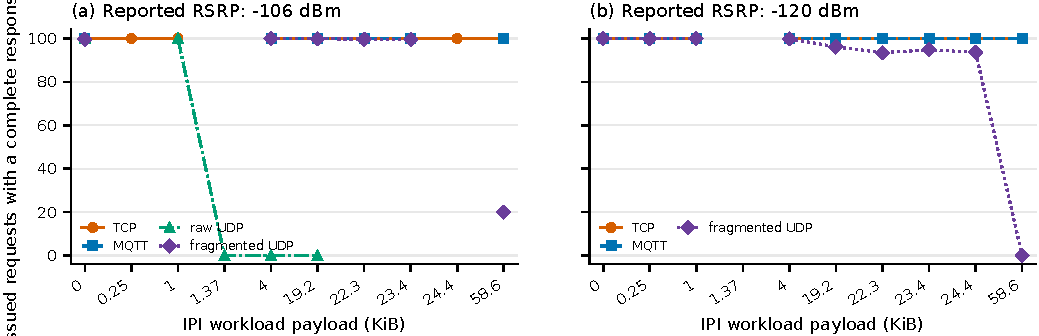
\includegraphics[width=\textwidth]{figs/section5_protocol_completion.pdf}
  \caption{Uplink-heavy response completion by transport, IPI workload size,
  and reported RSRP. Each line reports the percentage of issued requests that
  returned a complete response. A gap denotes an unevaluated transport-size
  pair. Fragmented UDP uses 1,400-B adapter-level fragments and completes a
  response only after reassembly.}
  \Description{Two line plots compare the percentage of issued requests that
  returned a complete response over TCP, MQTT, raw UDP, and fragmented UDP at
  reported RSRP values of minus 106 and minus 120 dBm. Line gaps identify
  transport-size pairs that were not evaluated.}
  \label{fig:protocol-results}
\end{figure*}

\subsection{5G Uplink: Transport Effects on Completion and Latency}
\label{sec:results-protocol}

Payload size determines how much application data the uplink must carry;
transport determines whether the encoded object is delivered as a stream or as
one or more datagrams. We therefore compare TCP, MQTT over TCP, raw UDP, and
UDP with adapter-level fragmentation at matched object sizes and field
conditions.
Figure~\ref{fig:protocol-results} compares empty-payload controls, detector-derived
payloads, and the 58.6-KiB stress payload. TCP and MQTT returned every response
at each size in the $-106$-dBm collection. At $-120$~dBm, their 58.6-KiB p95
RTTs exceeded 660~ms, and their p99 RTTs exceeded 1~s.

The detector sweep also gives a conservative size boundary for a 500-ms CAV
decision budget. Every evaluated TCP and MQTT condition through 19.2~KiB of
application payload had a p95 RTT below 500~ms in both the $-106$- and
$-120$-dBm collections. At 22.3~KiB, the $-120$-dBm MQTT p95 crossed the deadline at
539.780~ms. Later detector points fluctuated rather than restoring a monotonic
size guarantee. These measurements place the 500-ms p95 ceiling for this
uplink-heavy TCP/MQTT path at an approximately 20-KiB application payload
before transport framing. The ceiling appeared with one UE on a dedicated
40-MHz n48 channel and no ambient traffic.

Raw UDP completed the empty and 1-KiB conditions but returned no response for
the evaluated larger datagrams. Adapter-level fragmentation and receiver
reassembly sustained at least 93.5\% completion through 25~KiB. At 58.6~KiB,
completion fell to 20\% at $-106$~dBm and 0\% at $-120$~dBm. TCP and MQTT use
retransmission and buffering, while fragmented UDP loses more reassembled
responses as payload size and path difficulty grow.

\subsection{5G Uplink Across Stationary Radio Conditions}
\label{sec:results-signal-tdd}

After separating transport effects, the stationary comparison holds the
70/20/10 profile and uplink-heavy exchange fixed while compact and
detector-sized workloads run at four locations.
Figure~\ref{fig:signal-effects} plots the detector-sized results against the
reported RSRP at each location. The $-120$, pooled $-109$ to $-110$, and
$-101$~dBm blocks returned 5,994/6,000, 5,999/6,000, and 6,000/6,000 responses.
The larger $-109$ to $-110$-dBm campaign returned 307,662/309,000 responses.

\begin{figure}[t]
  \centering
  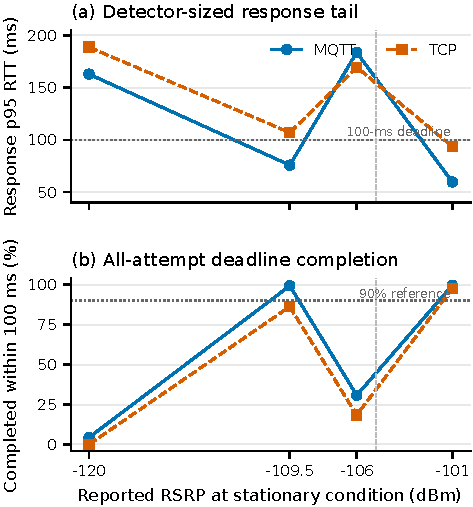
\includegraphics[width=\columnwidth]{figs/section5_signal_effects.pdf}
  \caption{Detector-sized uplink-heavy responses across four stationary
  70/20/10 conditions. (a) Response p95 RTT. (b) Percentage of all issued
  requests completed within 100~ms. The vertical line separates the weak and
  common/typical RSRP bins defined in Section~\ref{sec:setup}.}
  \Description{Two line plots compare MQTT and TCP detector-sized workload
  response p95 in milliseconds and the percentage of issued requests completed within 100
  milliseconds at four reported stationary RSRP values.}
  \label{fig:signal-effects}
\end{figure}

Compact 1-KiB exchanges change little within each transport. MQTT p95 spans
40.0--46.1~ms, and 99.1--100\% of issued requests complete within 100~ms. TCP
p95 spans 137.3--150.4~ms, with 0.5--4.6\% completion within 100~ms. The
detector-sized workload varies more. MQTT 100-ms completion is 4.4\%, 99.4\%,
30.8\%, and 99.7\% at $-120$, $-109$ to $-110$, $-106$, and $-101$~dBm. TCP
completion is 0\%, 86.3\%, 18.4\%, and 97.8\%. Across the same conditions,
MQTT p95 RTT is 162.9, 75.8, 183.7, and 59.7~ms; TCP p95 RTT is 188.7, 107.0,
169.5, and 93.6~ms.

The $-101$-dBm common/typical location produces the lowest detector-sized p95
and the highest 100-ms completion. The $-106$-dBm condition performs worse than
the pooled $-109$ to $-110$-dBm conditions, so RSRP alone does not order the
four outcomes. Payload size remains stable for the compact exchange and
sensitive to the broader radio and path conditions for detector-sized traffic.

\subsection{5G Downlink: Returned CAV Objects}
\label{sec:results-downlink}

The preceding campaigns place the larger application object on the uplink. We
next reverse the large-object direction. A downlink-heavy CAV operation begins
with a compact vehicle request and ends
after the vehicle receives and validates the returned application object. This
pattern represents raw sensor data, processed perception, planning data,
control data, or other state requested from an edge application. Under the
established 70/20/10 profile, the GL-X3000 downlink campaign returned all 4,000
TCP and all 4,000 MQTT responses across 1, 10, 100, and 500~KiB.

\begin{figure}[t]
  \centering
  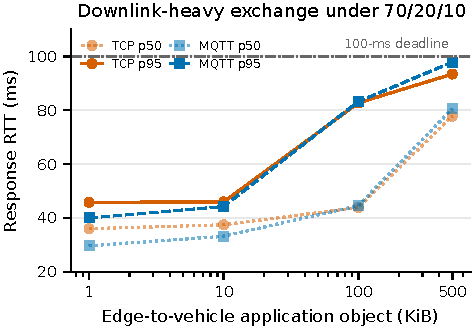
\includegraphics[width=\columnwidth]{figs/section5_downlink_latency.pdf}
  \caption{Downlink-heavy CAV object latency under the established 70/20/10
  profile. The vehicle sends a compact request and validates the complete
  1--500-KiB edge-to-vehicle object. Each point summarizes 500 exchanges.}
  \Description{A line plot shows TCP and MQTT median and 95th-percentile
  response round-trip time in milliseconds for edge-to-vehicle objects from 1
  to 500~KiB.}
  \label{fig:downlink-latency}
\end{figure}

Figure~\ref{fig:downlink-latency} shows p95 RTT rising from 45.8 to 93.4~ms for
TCP and from 40.0 to 97.8~ms for MQTT as the returned object grows from 1 to
500~KiB. The 500-KiB response tails remain below the 100-ms reference in this
stationary 70/20/10 condition. This established-profile result provides the
baseline for testing whether a different radio configuration preserves burst
latency and sustained-transfer goodput in both directions.

\subsection{5G TDD and Gateway Effects}
\label{sec:results-tdd-direction}

The TDD study evaluates whether the 40/40/20 behavior persists across vehicle
gateways. The MG52 campaigns measured both profiles, but route recovery,
serving-cell changes, and weaker signal accompanied part of the 40/40/20
collection. We therefore repeated the complete bidirectional matrix with a
GL-X3000 at one stationary location. Within this repeat, TDD is the changing
configuration; gateway, location, application, transport, and payload matrix
remain fixed.

\begin{figure*}[t]
  \centering
  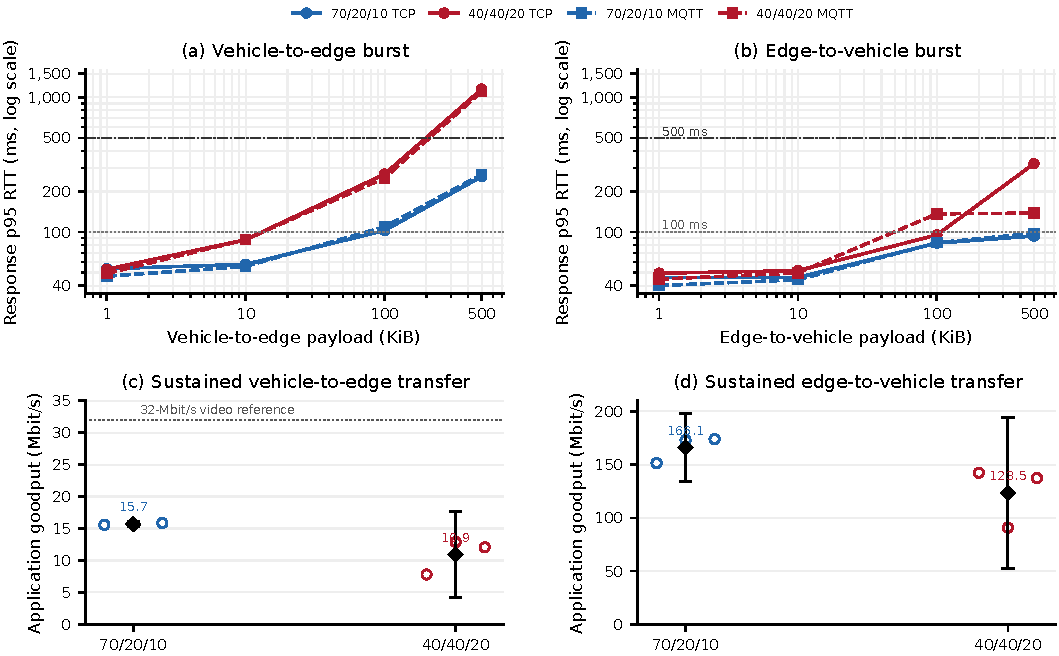
\includegraphics[width=\textwidth]{figs/section5_tdd_profiles.pdf}
  \caption{Same-device performance for CAV bursts and sustained transfers.
  The GL-X3000 blocks use the same stationary location;
  70/20/10 and 40/40/20 have median RSRP of $-99$ and $-98$~dBm and median
  SINR of 20~dB. Panels (a--b) combine TCP and MQTT p95 RTT; each
  profile-transport marker summarizes 500 validated exchanges. The
  dotted and dash-dotted lines mark 100- and 500-ms application references.
  Panel (c) combines three exact 50-MiB transfers per profile and direction on
  a logarithmic goodput axis; open circles are individual transfers, diamonds
  are means, and whiskers are $t$-based 95\% confidence intervals. The dotted
  line marks the 32-Mbit/s remote-teleoperation video reference.}
  \Description{Three panels compare 70/20/10 and 40/40/20 using one GL-X3000.
  Two panels combine TCP and MQTT p95 round-trip time in milliseconds for
  vehicle-to-edge and edge-to-vehicle objects from 1 to 500~KiB. The third
  panel compares receiver-observed upload and download goodput in Mbit/s.}
  \label{fig:tdd-profiles}
\end{figure*}

The GL-X3000 repeat contains 8,000 validated exchanges under each profile.
Every exchange returned a response. The profile difference appears in latency
rather than eventual completion.

At 1~KiB, vehicle-to-edge p50 RTT was effectively tied. The difference grew
with the vehicle-originated object. At 500~KiB, 40/40/20 increased TCP p50 RTT
from 231.046 to 609.652~ms. TCP p95 increased from 258.200 to
1,149.368~ms. MQTT p50 increased from 238.607 to 580.942~ms, while p95
increased from 267.336 to 1,104.331~ms. The corresponding p95 ratios were 4.45
and 4.13. Edge-to-vehicle objects also had higher p95 RTT under 40/40/20
at every evaluated size and transport. The 500-KiB ratios were 3.44 for TCP
and 1.41 for MQTT (Figure~\ref{fig:tdd-profiles}(a--b)).

These tail changes reduced deadline completion across the equally sized
workload matrix. Under 70/20/10, 14.54\%, 0.04\%, and 0\% of the 8,000
exchanges exceeded 100, 500, and 1,000~ms. Under 40/40/20, the corresponding
fractions were 30.85\%, 9.81\%, and 1.26\%. The latter profile produced 101
second-scale exchanges; 82 occurred in the two 500-KiB vehicle-to-edge
conditions. Thus, the alternative configuration widened the large-burst tail
even though it nominally assigns twice as much of the frame to fixed uplink
use.

The radio measurements place both profile blocks in the same signal category.
Median RSRP was $-99$~dBm under 70/20/10 and $-98$~dBm under 40/40/20. Median
SINR was 20~dB in both blocks. Restricting the analysis to their common
RSRP/SINR range retained 15,153 exchanges and the same latency ordering in 14
of 16 p50 comparisons and 15 of 16 p95 comparisons. At 500~KiB, TCP
vehicle-to-edge server processing remained 1.617--1.619~ms at p50 while
response RTT changed by 378.606~ms. The latency ordering therefore persists
within common measured signal support, while the endpoint processing time
remains nearly identical.

The exact transfers measure the sustained-stream component of CAV traffic.
Each profile completed three 50-MiB uploads and three 50-MiB downloads with
matching byte counts and checksums. Vehicle-to-edge goodput averaged
15.691~Mbit/s under 70/20/10. It averaged 10.913~Mbit/s under 40/40/20, a
30.4\% reduction. Edge-to-vehicle goodput averaged 166.106 and
123.451~Mbit/s, a 25.7\% reduction. Every 40/40/20 transfer was slower than every corresponding
70/20/10 transfer (Figure~\ref{fig:tdd-profiles}(c)). The two upload means
provide 49.0\% and 34.1\% of the 32-Mbit/s remote-teleoperation video reference
in Table~\ref{tab:application-envelopes}.

The cross-gateway controls separate device improvement from the profile
ordering. Under 70/20/10, GL-X3000 upload and download goodput exceeded the
closest MG52 control by 30.8\% and 31.0\%. The earlier MG52 large-uplink collapse
did not recur with the GL-X3000, but the same-device comparison still favored
70/20/10 for burst latency and sustained goodput. Earlier profile transitions
also changed route, cell state, and serving cell. Later matched blocks completed
their exchanges but retained configuration-dependent latency and goodput.
In this deployment, the evaluated 40/40/20 implementation was not ready for
deadline-sensitive CAV traffic. Its initial MG52 rollout was operationally
unstable, and its matched GL-X3000 repeat produced higher burst latency and lower
directional goodput than 70/20/10. The additional nominal uplink allocation did
not translate into predictable application performance.

\begin{figure}[t]
  \centering
  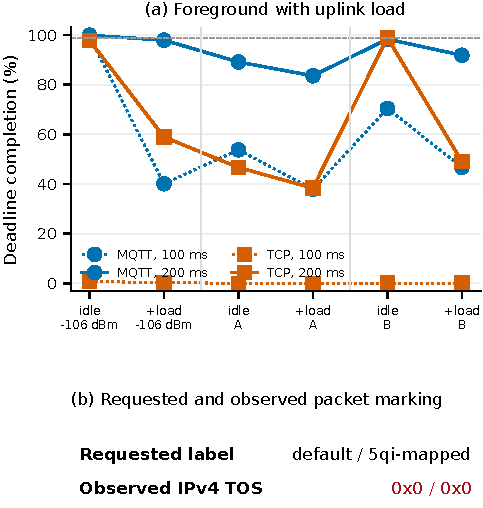
\includegraphics[width=\columnwidth]{figs/section5_mixed_load_qos.pdf}
  \caption{Compact foreground exchanges during a sustained uplink stream.
  (a) Percentage of issued 1-KiB requests completed within 100 and 200~ms at
  idle and with the uplink generator active; Collections A and B are separate
  weak-signal field collections. (b) Requested application labels and the observed vehicle-side
  Internet Protocol version 4 Type of Service (TOS) value.}
  \Description{One panel compares foreground deadline completion with and
  without an uplink generator. A second panel shows that the two requested
  application labels both produced IPv4 Type of Service zero.}
  \label{fig:mixed-results}
\end{figure}

\subsection{Concurrent Bursts and Sustained Streams}
\label{sec:results-mixed}

The configuration comparison uses one application flow at a time. During
remote teleoperation, a vehicle can sustain a video stream while faults,
control updates, or planning requests create additional
deadline-sensitive exchanges. The load experiment models this
communication pattern with a continuing vehicle-to-edge stream and a compact
1-KiB foreground exchange on the same host and UE. With the generator active,
MQTT $C(100\,\mathrm{ms})$ fell from 99.70\% to 40.15\%, while TCP
$C(200\,\mathrm{ms})$ fell from 97.90\% to 59.00\%. Across the load
collections, achieved background traffic ranged from 1.320 to 5.743~Mbit/s.
The active generator reduced foreground deadline completion before reaching
the offered rate.

The response tails show the same shift. In the $-106$-dBm repetitions, the active
generator increased MQTT p95 from 52--60 to 174--176~ms and TCP p95 from
162--194 to 388--420~ms. The response tail did not vary monotonically with the
number of streams, so achieved background rate alone does not predict
foreground latency.

The default and \texttt{5qi-mapped} labels both produced observed TOS values of
\texttt{0x0} in the vehicle
capture (Figure~\ref{fig:mixed-results}(b)). The foreground and background
flows entered the measured path without an observed packet-class difference
between the requested labels. The sustained stream therefore displaced a
compact exchange from its deadline before reaching the 32-Mbit/s video
reference, and the requested application label did not create observable
packet differentiation on the vehicle interface.

\begin{figure*}[t]
  \centering
  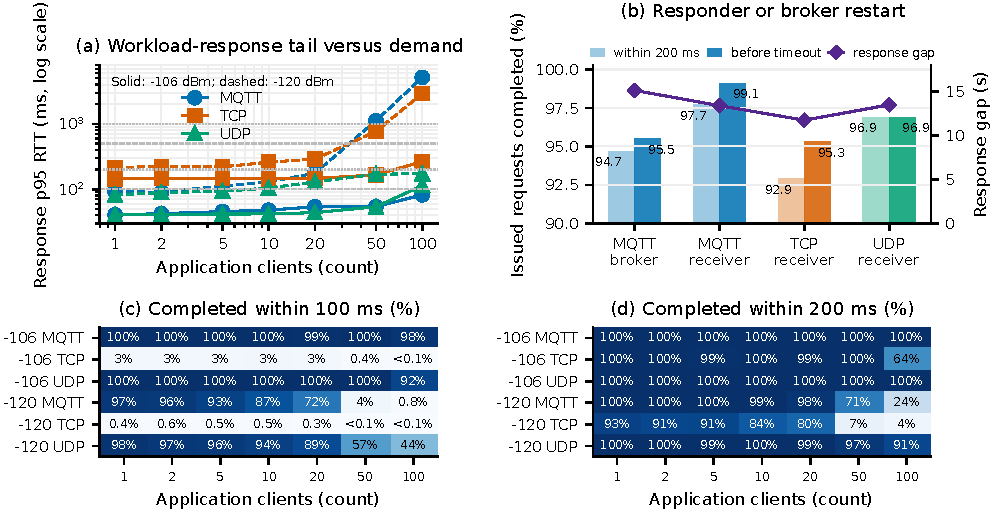
\includegraphics[width=0.99\textwidth]{figs/section5_concurrency_interruption.pdf}
  \caption{Client-demand and interruption results for 1-KiB application
  payloads. (a) Response p95 RTT in milliseconds versus client count; solid
  and dashed lines mark the $-106$-
  and $-120$-dBm weak-band collections. (b) Completion percentage within
  200~ms and before timeout, together with the response gap in
  seconds after a 10-s restart. (c--d) Percentages of all issued requests
  completed within 100 and 200~ms.}
  \Description{Four panels compare response latency and deadline completion as
  application clients increase, plus completion and response gaps during four
  endpoint or broker restarts.}
  \label{fig:concurrency-interruption}
\end{figure*}

\subsection{Concurrent Application Demand}
\label{sec:results-concurrency}

The preceding experiment combines one continuing stream with one foreground
exchange. CAVs can also start several perception, planning, and control
operations at the same time. The client-demand experiment increases the number
of simultaneous application flows behind the same physical UE.

The client-demand experiment scales a homogeneous 1-KiB exchange across
multiple application clients on one host and UE. At 100 clients and
$-106$~dBm, aggregate p95 RTT was 81.850~ms for MQTT, 264.070~ms for TCP, and
113.391~ms for UDP. At $-120$~dBm, MQTT and TCP p95 rose to 5,135.984 and
2,908.420~ms. UDP p95 was 172.500~ms, but 9,189 of 100,000 cycles received no
response. Figure~\ref{fig:concurrency-interruption}(c--d) shows that deadline
completion falls as client demand grows. Per-client tail distributions further
show that individual flows can miss the 100- and 200-ms budgets even when most
aggregate requests eventually receive a response.

\subsection{Endpoint Interruption and Recovery}
\label{sec:results-interruption}

The demand experiment varies concurrent flows while each endpoint remains
available. To measure recovery separately, the interruption experiment
restarted a receiver or broker for 10~s while
1-KiB requests continued. MQTT broker, MQTT receiver, TCP receiver, and UDP
receiver restarts returned 955/1,000, 991/1,000, 953/1,000, and 969/1,000
responses. At the 200-ms remote-assistance budget, completion was 94.7\%,
97.7\%, 92.9\%, and 96.9\%. The gaps between received responses were 15.1007,
13.3674, 11.7147, and 13.4635~s. Every response gap exceeds the injected
outage and is absent from response-only latency percentiles. Among the
responses that arrived, the corresponding p99 RTTs were
90.553, 259.906, 361.228, and 63.027~ms.

\subsection{Cross-Application Comparison}
\label{sec:results-cross-application}

The preceding subsections report path-specific response latency and deadline
completion. Figure~\ref{fig:cross-application} places the p50, p95, and maximum
RTT of each selected condition beside its application deadline. Each response
marker is green when it meets the deadline and red when it exceeds the
deadline.

\begin{figure*}[t]
  \centering
  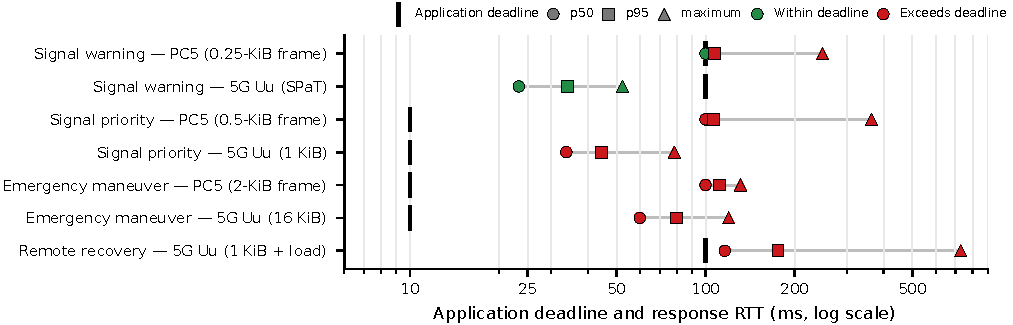
\includegraphics[width=\textwidth]{figs/section5_cross_application_comparison.pdf}
  \caption{Application deadlines and measured response distributions. Each
  black tick is the deadline from Table~\ref{tab:application-envelopes}.
  Circles, squares, and triangles show response p50, p95, and maximum RTT;
  green markers meet the deadline and red markers exceed it. Row labels state
  the path and workload size used for each comparison. PC5 row labels report
  complete serialized IPI frame size; Uu row labels report application-object
  size.}
  \Description{A horizontal log-scale comparison places application deadlines
  and measured response median, 95th-percentile, and maximum round-trip times
  in milliseconds on the same row. Green markers meet the deadline and red
  markers exceed it.}
  \label{fig:cross-application}
\end{figure*}

The 5G MQTT SPaT exchange has p50, p95, and maximum RTTs of 23.4, 34.1, and
52.4~ms, so its complete measured distribution remains within the 100-ms
signal-warning deadline. The stationary 0.25-KiB PC5 frame exchange has a 100.0-ms
p50, a 106.9-ms p95, and a 248.6-ms maximum; only its median remains within the
same deadline. Both signal-priority conditions and both emergency-maneuver
conditions exceed their 10-ms deadlines at p50. The loaded 1-KiB remote-
recovery condition also exceeds its 100-ms deadline at p50, p95, and maximum,
which reach 116.1, 175.9, and 729.8~ms.

Operating conditions also alter the same workload when payload and deadline
are held fixed. For the detector-sized workload under 70/20/10,
100-ms MQTT completion is 4.4\% at $-120$~dBm. It reaches 99.7\% at the
common/typical location with $-101$~dBm recorded RSRP. The $-106$-dBm
70/20/10 condition reaches 30.8\%. Thus, the same profile and workload cross
the application deadline as location changes.

The measured deadline outcome also differed between the two deployed
configurations within the same signal category. In the GL-X3000 comparison, the fraction of
all exchanges exceeding 500~ms increased from 0.04\% under 70/20/10 to 9.81\%
under 40/40/20. The latter configuration also reduced sustained upload and
download goodput by 30.4\% and 25.7\%. The corresponding RSRP medians differed
by 1~dB, and both blocks had 20-dB median SINR.

Shared demand changes the same deadline a second way. Compact 1-KiB MQTT completion falls
from 99.7\% to 40.15\% with competing uplink traffic
(Figure~\ref{fig:mixed-results}(a)) and from 96.6\% to 0.751\% as $-120$-dBm
client demand grew from one to 100
(Figure~\ref{fig:concurrency-interruption}(c)). The default and
\texttt{5qi-mapped} labels both produced vehicle-side TOS \texttt{0x0}.
Consequently, the measured path exposed no packet-class distinction between
these labels as competing traffic and concurrent application demand moved the
same 1-KiB workload across its deadline.

\FloatBarrier
\subsection{Summary and Insights}
\label{sec:results-insights}

The cross-application comparison identifies different payload, coverage,
direction, radio-configuration, and demand limits. CAV traffic can begin with
an event-triggered uplink or downlink burst and then continue as a sustained
stream during remote teleoperation or continuing sensor delivery. Other
deadline-sensitive operations can begin while that stream remains active.
Increasing the workload and varying the operating conditions reveal where each
path crosses the application deadline and how many issued requests remain
within it. These measured boundaries lead to three insights:

\begin{enumerate}
  \renewcommand{\labelenumi}{\arabic{enumi})}
  \item \textbf{The measured commercial direct V2X path supports compact J2735
  messages only within a limited payload and coverage envelope.} The 68-m
  building-obstructed point lost every 1- and 2-KiB exchange, whereas the 113-m
  point completed 99.8--100\% of each tested frame size. Deployment planning
  must therefore account for obstruction and road geometry when placing RSUs
  or supplemental paths.

  \item \textbf{The measured 5G uplink supports only severely limited CAV
  packet sizes within decision deadlines.} The conservative
  500-ms p95 ceiling was approximately 20~KiB, and only 37.76\% of issued
  requests at or below 4~KiB completed within 100~ms. These limits appeared on
  a dedicated 40-MHz channel with one UE and no ambient contention. Because
  matched large objects had much longer uplink than downlink tails, CAV
  developers need direction-specific packet budgets and must reduce or
  progressively transmit vehicle-originated state when necessary.

  \item \textbf{5G/6G systems must support event-triggered CAV bursts,
  sustained directional streams, and concurrent deadline-sensitive traffic.}
  In the same-device comparison, 40/40/20 produced more deadline misses and
  lower sustained goodput than 70/20/10 despite its larger nominal uplink
  allocation. A sustained uplink stream also moved compact foreground
  exchanges across their deadlines. Radio vendors and mobile network operators
  must validate balanced and uplink-oriented configurations across radios and
  vehicle gateways, while schedulers isolate simultaneous flows by direction,
  deadline, and duration.
\end{enumerate}
